\documentclass{article}

\usepackage[margin=1in]{geometry}
\usepackage{verbatim}
\usepackage{graphicx}

\setlength\parindent{0pt}
\title{Basic \LaTeX Formatting}
\author{John Doe}
\date{}

\begin{document}
\maketitle
\section{Introduction}

Basic formatting tags in \LaTeX

\subsection{Text Formatting}

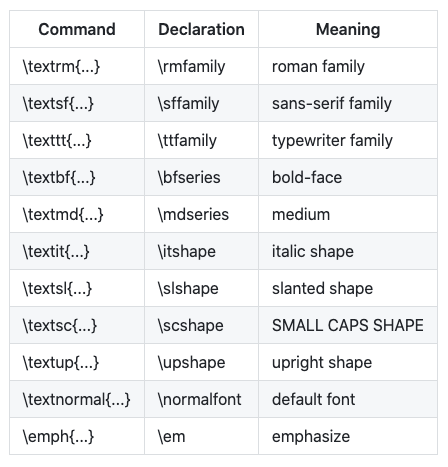
\includegraphics[scale=0.5]{image/commands.png}

{\sffamily
	Text is sans-serif. Text can be {\em emphasized}.
}

Normal text, {\sffamily sans serif text {\bfseries and bold}}.

\textbf{Bold formatting}

{\bfseries Text to bold}

\bfseries Text to bold \mdseries

\emph{Italics formatting}

\textit{italic}

\textsl{slanted}

\textsc{Small Caps}

% can be nested
\textit{\textbf{nested}}

\underline{Underline formatting}

\subsection{Paragraph formatting}

New paragraph are automatically indented.

\noindent But you can use noindent.

\section{Oddities}

Direction of single and double quotes.

\subsection{Misquoting}

Using 'single' and "double" quoting.
\\

\noindent But you can use a backtick, `single quote' and ``double quote".


\section{Fonts}

% Use this for source codes
\texttt{typewriter font}

\textsf{sans-serif}

section{\textsf{\LaTeX\ resources on the internet}}

\textrm{Roman fonts}



\section{Indent}

Paragraphs will be automatically indented.

\begin{verbatim}
Use \setlength\parindent{0pt} for noindent throughout the document.

Use \noindent for part of document.

\end{verbatim}

\section{Columns}
\begin{verbatim}
Use \documentclass{proc} for two columns format.
\end{verbatim}

\subsection{Commenting}
\begin{verbatim}
Use % for comments.

\end{verbatim}

\subsection{Other notes}
\begin{verbatim}
'\,' 1\,cm
\end{verbatim}

\end{document}

